% Provenance (never printed): see sources/outline_sources.md (Year 2: field and laboratory methods ---
% igneous and metamorphic petrography, chemical analysis by XRF, ICP-MS and microprobe, isotope mass
% spectrometry, a mapping campaign). Modelled on Book 3 ch. 6.
% Textures: BGS RR 99-02 (Robertson 1999), Open University Virtual Microscope, Carleton BH250,
% UCSB Geology 102C (Hacker); QAPF: BGS RR 99-06 (Gillespie and Styles 1999); instruments: SERC
% Geochemical Instrumentation and Analysis sheets (EPMA, WDS, XRF, TIMS, MC-ICPMS); XRF procedure
% and reference-material results: USGS OFR 02-223 and its chapter T (Taggart and Siems 2002); Sr
% isotopes: CIAAW; spike and mass bias: Cheong, Jeong and Kwon (2014). Ledger rows in
% sources/ledger/book4.md; curves and stations from figdata/bachelor-2/labmethods.py, numbers from
% the Book 4 second-writer scratch calculator calc/ch31.py. Observation only: the professional work
% is described in the third person.
\chapter{Metode Lapangan dan Laboratorium II}\label{ch:b2:field-lab-methods-2}

Setiap angka dalam bab-bab petrologi buku ini berawal sebagai batuan di dalam kantong, sayatan tipis di bawah
mikroskop, dan serbuk di dalam suatu instrumen. Komposisi mineral yang diplot pada diagram fase, kandungan
silika yang menamai suatu lava, rasio isotop stronsium yang melacak suatu sumber mantel: masing-masing
keluar dari rangkaian operasi yang dimulai di suatu singkapan, dan masing-masing membawa galat dari setiap
mata rantainya. Bab ini mengikuti rangkaian itu untuk batuan dasar Perbukitan Varden: membaca tekstur
dalam sayatan tipis, menghitung mineral, menganalisis batuan utuh, lalu mineral tunggal, lalu isotop,
dan pada setiap langkah menanyakan seberapa baik angka itu.

\begin{recall}
\textbf{Dari volume Tahun 1}: stasiun lapangan dan buku catatan lapangan, sampel terorientasi dan sayatan tipis,
mikroskop polarisasi, cahaya terpolarisasi bidang, polarisasi silang; identifikasi optis mineral
pembentuk batuan; penghitungan ulang rumus mineral dari analisis oksida pada jumlah oksigen yang tetap,
dan besi feri dengan keseimbangan muatan; foliasi dan skistositas; isokron, rasio awal, dan
garis kuadrat terkecil. \textbf{Dari buku-buku kimia}: spektrometri massa, plasma gandeng induktif;
kurva kalibrasi, batas deteksi dan batas kuantifikasi, presisi, kebenaran dan bias,
keterulangan, simpangan baku rata-rata. \textbf{Dari buku-buku fisika}: sinar-X karakteristik
dan hukum Moseley; hukum Bragg; tegangan permukaan; perambatan ketidakpastian.
\textbf{Dari buku-buku matematika}: distribusi binomial, rata-rata dan variansnya.
\textbf{Dari \cref{ch:b2:magmatic-series}}: \omterm{def:b2:magmatic-series:qapf}{komposisi modal}, \omterm{def:b2:magmatic-series:qapf}{diagram QAPF}.
\textbf{Dari \cref{ch:b2:isotope-geochemistry}}: \omterm{def:b2:isotope-geochemistry:tracer}{pelacak isotop radiogenik}, \omterm{def:b2:isotope-geochemistry:standards}{standar acuan isotop}.
\end{recall}

\section{Petrografi: tekstur sebagai sejarah}\label{sec:b2:field-lab-methods-2:petrography}

Volume Tahun 1 memakai mikroskop polarisasi untuk mengidentifikasi mineral. Seorang petrograf juga membaca
cara butir-butir tersusun, karena susunan itu merekam urutan pertumbuhannya. Dua
tekstur merupakan saksi yang paling umum dari kristalisasi dari lelehan dan dari rekristalisasi dalam
keadaan padat.

\begin{definition}[Tekstur ofitik, tekstur granoblastik]\label{def:b2:field-lab-methods-2:textures}
Suatu batuan beku dikatakan memiliki \emph{tekstur ofitik}\index{tekstur ofitik} bila kristal-kristal piroksen yang besar
melingkupi bilah-bilah plagioklas kecil yang berorientasi acak; tekstur ini khas bagi dolerit, gabro,
dan basal. Suatu batuan metamorf dikatakan memiliki \emph{tekstur granoblastik}\index{tekstur granoblastik} bila batuan itu
merupakan agregat kristal-kristal yang kurang lebih sama dimensi dan berukuran hampir sama, dalam banyak kasus anhedral,
yang batas-batas lurusnya bertemu bertiga pada sudut di dekat \ang{120}.
\end{definition}
% ledger: carletonB:ophitic, ouVM:textures, bgsM:textures

Dalam batuan ofitik, bilah-bilah yang terlingkupi itu utuh dan euhedral, dan piroksen mengisi ruang
di antaranya: plagioklas tumbuh lebih dahulu, piroksen di sekelilingnya. Sudut \ang{120} pada
\omterm{def:b2:field-lab-methods-2:textures}{tekstur granoblastik} adalah sudut butir-butir yang telah sempat menyesuaikan batas-batasnya; bahan ajar petrografi membaca sambungan
rangkap tiga semacam itu sebagai tanda kesetimbangan kimia dan tekstur. Sudut itu berasal dari keseimbangan gaya, dengan batas-batas butir menarik garis
persekutuannya seperti selaput sabun (tegangan permukaan, dari buku-buku fisika).
% ledger: ouVM:equilibrium

\begin{proposition}[Sudut-sudut pada sambungan rangkap tiga]\label{prop:b2:field-lab-methods-2:triple}
Misalkan tiga batas butir bertemu di sepanjang suatu garis, dengan tegangan (energi per satuan luas) $\gamma_1$,
$\gamma_2$, $\gamma_3$, dan misalkan $\theta_i$ adalah sudut antara dua batas selain
batas $i$. Pada kesetimbangan,
\begin{equation}
\frac{\gamma_1}{\sin\theta_1} = \frac{\gamma_2}{\sin\theta_2} = \frac{\gamma_3}{\sin\theta_3},
\label{eq:b2:field-lab-methods-2:lami}
\end{equation}
dan tiga tegangan yang sama bertemu pada tiga sudut \ang{120}.
\end{proposition}

\begin{proof}
Pada bidang yang tegak lurus terhadap sambungan itu, setiap batas menarik sambungan di sepanjang jejaknya sendiri
dengan gaya $\gamma_i$ per satuan panjang. Pada kesetimbangan ketiga gaya itu berjumlah nol, sehingga bila disusun
ujung ke pangkal, ketiganya menutup sebuah segitiga. Sudut segitiga di hadapan sisi $\gamma_i$ adalah
$\pi - \theta_i$, yang sinusnya $\sin\theta_i$, dan aturan sinus dalam segitiga itu memberikan
\eqref{eq:b2:field-lab-methods-2:lami}. Jika ketiga tegangan sama, segitiga itu
sama sisi, dan setiap sudut luar $\theta_i$ adalah $\pi - \pi/3 = 2\pi/3$, yaitu \ang{120}.
\end{proof}

\begin{omfigure}
\centering
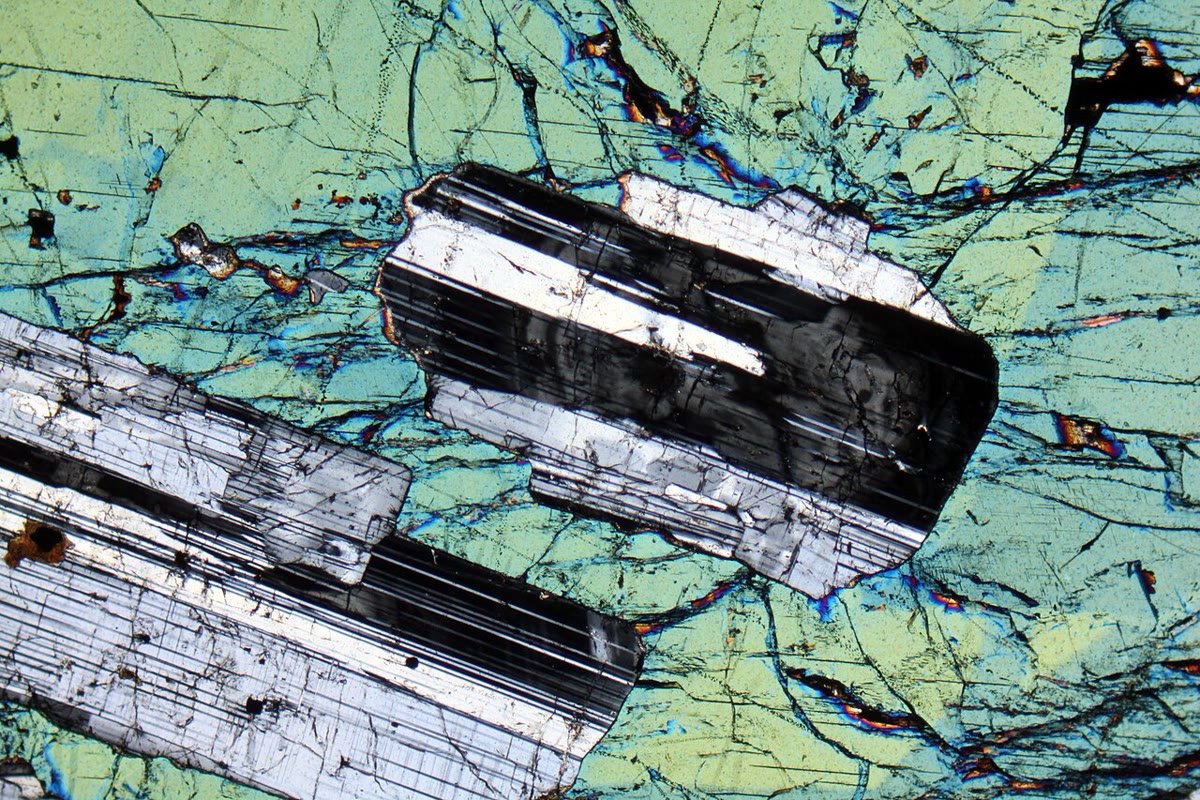
\includegraphics[height=4.6cm]{images/book4/b2-31-ophitic.jpg}\quad
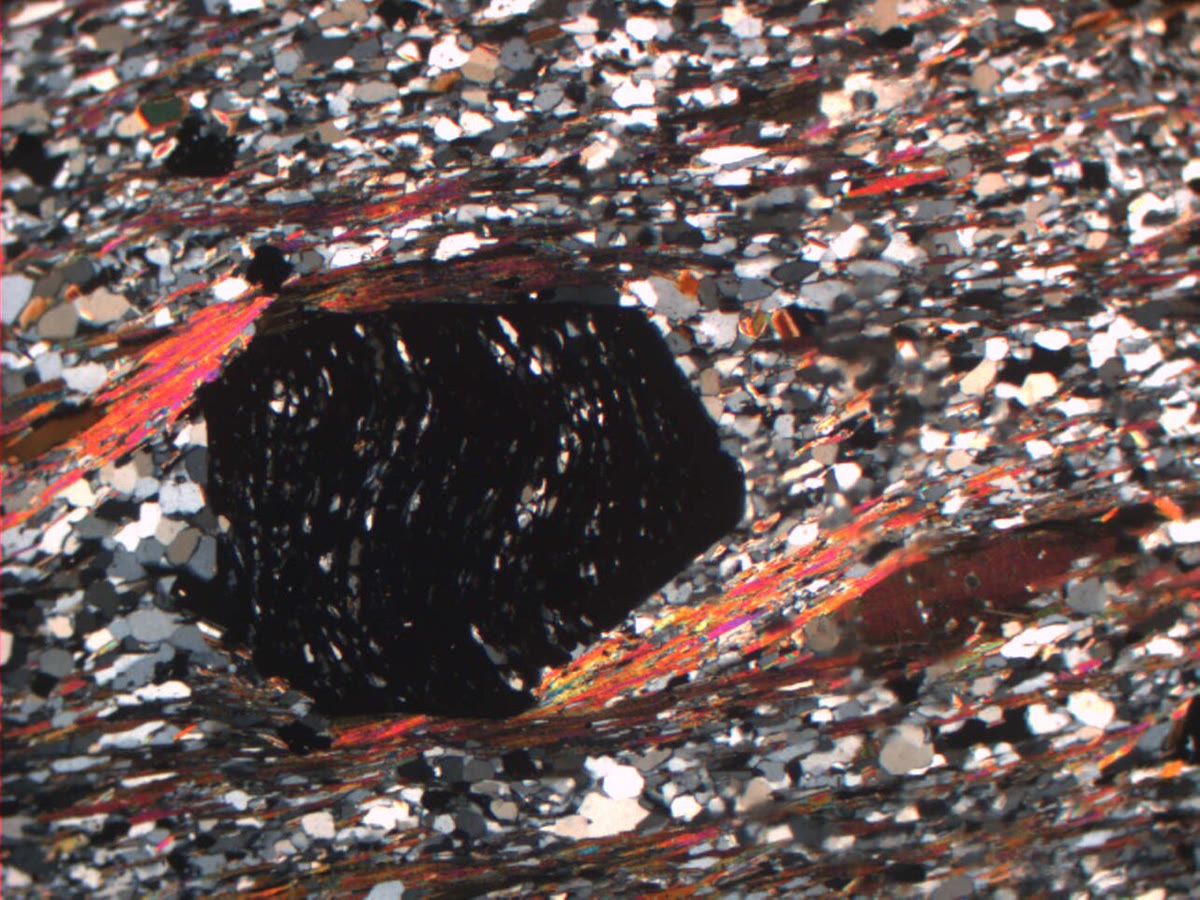
\includegraphics[height=4.6cm]{images/book4/b2-31-garnet-porphyroblast.jpg}
\par\smallskip{\small Dua tekstur di antara polarisator bersilang. Kiri: satu kristal augit (biru
dan hijau) melingkupi bilah-bilah plagioklas yang bergaris oleh kembarannya, susunan \omterm{def:b2:field-lab-methods-2:textures}{tekstur
ofitik}; medan pandang \qty{7}{mm}. Foto Strekeisen, CC BY-SA 4.0 (Wikimedia Commons).
Kanan: sekis garnet--mika. Garnet, hitam karena isotropik, adalah kristal besar yang
tumbuh dalam keadaan padat; inklusi kuarsa memotongnya dalam jejak-jejak, dan foliasi muskovit
(warna cerah), biotit (cokelat), dan kuarsa (abu-abu) melengkung di sekelilingnya. Foto Jackdann88,
CC BY 3.0 (Wikimedia Commons).}
\end{omfigure}
% ledger: photo:b2-31-ophitic, photo:b2-31-garnet

Mineral metamorf tidak semuanya tumbuh dengan laju yang sama. Sebagian spesies tumbuh melampaui yang lain menjadi kristal yang sangat besar,
yang menelan butir-butir kecil di sekitarnya selama tumbuh.

\begin{definition}[Porfiroblas, poikiloblas, jejak inklusi, korona]\label{def:b2:field-lab-methods-2:porphyroblast}
Yang disebut \emph{porfiroblas}\index{porfiroblas} adalah kristal besar yang tumbuh selama \omterm{def:b2:metamorphic-facies:metamorphism}{metamorfisme}
di dalam massa dasar yang lebih halus; garnet, staurolit, kordierit, dan kloritoid membentuknya, dari
beberapa milimeter sampai beberapa sentimeter lebarnya. Yang disebut \emph{poikiloblas}\index{poikiloblas} adalah
porfiroblas yang mengandung banyak inklusi mineral lain. Yang disebut \emph{jejak
inklusi}\index{jejak inklusi} adalah deretan inklusi yang sejajar di dalam suatu porfiroblas, yang
mengawetkan fabrik massa dasar pada saat kristal itu tumbuh melampauinya. Yang disebut
\emph{korona}\index{korona (tekstur reaksi)} adalah tepian satu atau lebih mineral baru yang sepenuhnya
mengelilingi suatu mineral yang sedang terurai, karena mineral itu tidak lagi stabil bersama
tetangga-tetangganya: suatu tekstur reaksi, yang membeku sebelum reaksinya selesai.
\end{definition}
% ledger: bgsM:textures, ouVM:textures

Membandingkan \omterm{def:b2:field-lab-methods-2:porphyroblast}{jejak inklusi} ($S_i$, fabrik internal) dengan foliasi di luar kristal
($S_e$, fabrik eksternal) menentukan umur pertumbuhan suatu \omterm{def:b2:field-lab-methods-2:porphyroblast}{porfiroblas} relatif terhadap deformasi yang
membentuk foliasi itu. Kriteria di bawah, yang digambar pada gambar, adalah kriteria catatan ajar baku.
% ledger: ucsbH:inclusion-trails

\begin{method}[Menentukan waktu pertumbuhan porfiroblas dari jejak inklusinya]\label{met:b2:field-lab-methods-2:timing}
Carilah sayatan yang dipotong tegak lurus terhadap foliasi, lalu bandingkan $S_i$ dan $S_e$.
\begin{enumerate}
  \item \textbf{Inklusi acak}, $S_e$ terbelokkan di sekeliling kristal: kristal tumbuh sebelum
        foliasi terbentuk (\emph{pra-tektonik}).
  \item \textbf{$S_i$ lurus yang terpotong di tepian}, tidak menerus dengan $S_e$ yang terbelokkan: kristal tumbuh
        di atas foliasi yang lebih tua, di antara dua deformasi (\emph{inter-tektonik}).
  \item \textbf{$S_i$ melengkung}, menerus dengan $S_e$: kristal tumbuh selagi foliasi terbentuk, sambil berotasi
        atau ditumbuhi selagi tumbuh (\emph{sin-tektonik}; spiral garnet bola salju).
  \item \textbf{$S_i$ lurus yang menerus dengan $S_e$ yang tidak terbelokkan}: kristal tumbuh setelah foliasi
        (\emph{pasca-tektonik}).
\end{enumerate}
\end{method}

\begin{omfigure}
\centering
\begin{tikzpicture}[x=1cm, y=1cm, font=\scriptsize]
% schematic after the criteria of ledger ucsbH:inclusion-trails
% panel 1: pre-tectonic
\begin{scope}[shift={(0,0)}]
\draw[omExo, line width=0.5pt] (-1.5,0.95) .. controls (-0.6,0.95) and (-0.5,0.85) .. (0,0.85) .. controls (0.5,0.85) and (0.6,0.95) .. (1.5,0.95);
\draw[omExo, line width=0.5pt] (-1.5,-0.95) .. controls (-0.6,-0.95) and (-0.5,-0.85) .. (0,-0.85) .. controls (0.5,-0.85) and (0.6,-0.95) .. (1.5,-0.95);
\draw[omExo, line width=0.5pt] (-1.5,0.45) .. controls (-0.9,0.45) and (-0.85,0.78) .. (0,0.78) .. controls (0.85,0.78) and (0.9,0.45) .. (1.5,0.45);
\draw[omExo, line width=0.5pt] (-1.5,-0.45) .. controls (-0.9,-0.45) and (-0.85,-0.78) .. (0,-0.78) .. controls (0.85,-0.78) and (0.9,-0.45) .. (1.5,-0.45);
\draw[omExo, line width=0.5pt] (-1.5,0) -- (-0.78,0); \draw[omExo, line width=0.5pt] (0.78,0) -- (1.5,0);
\filldraw[fill=omThm!15, draw=omThm, line width=0.6pt] (0,0) circle (0.72);
\draw[black, line width=0.7pt] (-0.4,0.2) -- (-0.25,0.35); \draw[black, line width=0.7pt] (0.1,0.35) -- (0.3,0.2);
\draw[black, line width=0.7pt] (-0.35,-0.2) -- (-0.15,-0.25); \draw[black, line width=0.7pt] (0.2,-0.15) -- (0.25,-0.4);
\draw[black, line width=0.7pt] (-0.05,0.05) -- (0.05,-0.1); \draw[black, line width=0.7pt] (0.35,0.0) -- (0.5,0.12);
\node at (0,-1.3) {pra-tektonik};
\end{scope}
% panel 2: inter-tectonic
\begin{scope}[shift={(3.4,0)}]
\draw[omExo, line width=0.5pt] (-1.5,0.95) .. controls (-0.6,0.95) and (-0.5,0.85) .. (0,0.85) .. controls (0.5,0.85) and (0.6,0.95) .. (1.5,0.95);
\draw[omExo, line width=0.5pt] (-1.5,-0.95) .. controls (-0.6,-0.95) and (-0.5,-0.85) .. (0,-0.85) .. controls (0.5,-0.85) and (0.6,-0.95) .. (1.5,-0.95);
\draw[omExo, line width=0.5pt] (-1.5,0.45) .. controls (-0.9,0.45) and (-0.85,0.78) .. (0,0.78) .. controls (0.85,0.78) and (0.9,0.45) .. (1.5,0.45);
\draw[omExo, line width=0.5pt] (-1.5,-0.45) .. controls (-0.9,-0.45) and (-0.85,-0.78) .. (0,-0.78) .. controls (0.85,-0.78) and (0.9,-0.45) .. (1.5,-0.45);
\draw[omExo, line width=0.5pt] (-1.5,0) -- (-0.78,0); \draw[omExo, line width=0.5pt] (0.78,0) -- (1.5,0);
\filldraw[fill=omThm!15, draw=omThm, line width=0.6pt] (0,0) circle (0.72);
\begin{scope}
\clip (0,0) circle (0.66);
\foreach \k in {-0.6,-0.3,0,0.3,0.6} {\draw[black, line width=0.7pt, dash pattern=on 2pt off 1.5pt] (-0.8,\k-0.45) -- (0.8,\k+0.45);}
\end{scope}
\node at (0,-1.3) {inter-tektonik};
\end{scope}
% panel 3: syn-tectonic
\begin{scope}[shift={(6.8,0)}]
\draw[omExo, line width=0.5pt] (-1.5,0.8) -- (1.5,0.8);
\draw[omExo, line width=0.5pt] (-1.5,-0.8) -- (1.5,-0.8);
\draw[omExo, line width=0.5pt] (-1.5,0.4) -- (-0.6,0.4); \draw[omExo, line width=0.5pt] (0.6,0.4) -- (1.5,0.4);
\draw[omExo, line width=0.5pt] (-1.5,0) -- (-0.72,0); \draw[omExo, line width=0.5pt] (0.72,0) -- (1.5,0);
\draw[omExo, line width=0.5pt] (-1.5,-0.4) -- (-0.6,-0.4); \draw[omExo, line width=0.5pt] (0.6,-0.4) -- (1.5,-0.4);
\filldraw[fill=omThm!15, draw=omThm, line width=0.6pt] (0,0) circle (0.72);
\draw[black, line width=0.7pt, dash pattern=on 2pt off 1.5pt] (-0.6,0.4) .. controls (-0.35,0.4) and (-0.2,0.3) .. (-0.05,0.4) .. controls (0.1,0.5) and (0.35,0.4) .. (0.6,0.4);
\draw[black, line width=0.7pt, dash pattern=on 2pt off 1.5pt] (-0.72,0) .. controls (-0.3,0) and (-0.3,-0.45) .. (0,0) .. controls (0.3,0.45) and (0.3,0) .. (0.72,0);
\draw[black, line width=0.7pt, dash pattern=on 2pt off 1.5pt] (-0.6,-0.4) .. controls (-0.35,-0.4) and (-0.1,-0.5) .. (0.05,-0.4) .. controls (0.2,-0.3) and (0.35,-0.4) .. (0.6,-0.4);
\node at (0,-1.3) {sin-tektonik};
\end{scope}
% panel 4: post-tectonic
\begin{scope}[shift={(10.2,0)}]
\foreach \k in {-0.8,-0.4,0,0.4,0.8} {\draw[omExo, line width=0.5pt] (-1.5,\k) -- (1.5,\k);}
\filldraw[fill=omThm!15, draw=omThm, line width=0.6pt] (0,0) circle (0.72);
\begin{scope}
\clip (0,0) circle (0.66);
\foreach \k in {-0.8,-0.4,0,0.4,0.8} {\draw[black, line width=0.7pt, dash pattern=on 2pt off 1.5pt] (-0.8,\k) -- (0.8,\k);}
\end{scope}
\node at (0,-1.3) {pasca-tektonik};
\end{scope}
\end{tikzpicture}
\par\smallskip{\small \omterm{def:b2:field-lab-methods-2:porphyroblast}{Jejak inklusi} (hitam, putus-putus) di dalam \omterm{def:b2:field-lab-methods-2:porphyroblast}{porfiroblas} (merah) dan foliasi
di luarnya (abu-abu), dalam sayatan yang tegak lurus terhadap foliasi (skematis). Dari kiri ke kanan:
inklusi yang tumbuh sebelum foliasi, yang melengkung di sekeliling kristal; fabrik tua yang lurus dan terpotong
di tepian; jejak yang melengkung masuk ke dalam foliasi, karena kristal berotasi selama tumbuh; dan
jejak lurus yang melanjutkan foliasi yang tidak terganggu.}
\end{omfigure}

Petrografi juga bersifat kuantitatif. Proporsi mineral dalam batuan beku berbutir kasar
menamai batuan itu pada \omterm{def:b2:magmatic-series:qapf}{diagram QAPF} (\cref{ch:b2:magmatic-series}), dan proporsi itu diukur di bawah
mikroskop.

\begin{definition}[Analisis modal, penghitungan titik]\label{def:b2:field-lab-methods-2:modal}
Yang disebut \emph{analisis modal}\index{analisis modal} adalah pengukuran \omterm{def:b2:magmatic-series:qapf}{komposisi modal} suatu
batuan. Dalam \emph{penghitungan titik}\index{penghitungan titik}, sayatan
tipis digeser di bawah benang silang mikroskop dengan langkah yang sama di sepanjang kisi yang teratur, dan
mineral di bawah benang silang dicatat pada setiap titik; proporsi titik yang
jatuh pada suatu mineral menaksir proporsinya di dalam batuan.
\end{definition}

\begin{proposition}[Apa yang diukur penghitungan titik, dan seberapa baik]\label{prop:b2:field-lab-methods-2:counting}
(a) Dalam batuan tanpa orientasi pilihan, fraksi luas suatu mineral dalam sayatan yang diletakkan
secara acak, rata-rata, bernilai sama dengan fraksi volumenya. (b) Jika $n$ titik jatuh secara saling bebas
pada mineral dengan fraksi luas $p$, proporsi terhitung $\hat p = k/n$ memiliki rata-rata $p$ dan simpangan
baku
\begin{equation}
\sigma = \sqrt{\frac{p(1-p)}{n}} , \qquad\text{sehingga}\qquad n = \frac{p(1-p)}{\sigma^2}
\label{eq:b2:field-lab-methods-2:binomial}
\end{equation}
titik diperlukan untuk mencapai simpangan baku $\sigma$.
\end{proposition}

\begin{proof}
(a) Potonglah satu blok batuan setinggi $H$ menjadi sayatan-sayatan sejajar seluas $S$. Volume
mineral itu adalah $\int_0^H a(z)\,\mathrm{d}z$, dengan $a(z)$ luasnya dalam sayatan pada ketinggian $z$;
dengan membaginya dengan volume $SH$, fraksi volume adalah rata-rata fraksi luas $a(z)/S$ atas
semua ketinggian, yaitu nilai harapan untuk ketinggian yang diambil secara acak. (b) Setiap titik jatuh pada
mineral itu dengan probabilitas $p$, saling bebas dari yang lain, sehingga banyaknya kena $k$ mengikuti
distribusi binomial dengan parameter $n$ dan $p$, dengan rata-rata $np$ dan varians $np(1-p)$. Pembagian dengan
$n$ memberikan rata-rata $p$ dan varians $p(1-p)/n$ bagi $\hat p$.
\end{proof}

Bukti (b) mengandaikan titik-titik yang saling bebas, yang didekati oleh langkah kisi yang lebih besar daripada
butir. Untuk mineral yang menyusun \qty{30}{\percent} suatu batuan, 500 titik memberikan $\sigma =
\sqrt{0.3 \times 0.7/500} = 0.020$, dua poin persentase; mencapai satu poin persentase memerlukan
$0.21/0.01^2 = 2100$ titik, empat kali lebih banyak, karena $\sigma$ hanya turun sebagai $1/\sqrt n$.
Galat relatif, $\sigma/p = \sqrt{(1-p)/(np)}$, paling buruk untuk mineral yang jarang (gambar di bawah,
kiri). Proporsi terhitung lalu dihitung ulang untuk menamai batuan: suatu mode dengan
\qty{10}{\percent} kuarsa, 30 feldspar alkali, 20 plagioklas, dan 40 mineral mafik memberikan Q, A, dan
P sebesar 16.7, 50.0, dan 33.3 setelah ketiga komponen felsik dijadikan berjumlah 100. Pada segitiga
QAP, batuan dengan Q antara 20 dan 60 adalah granit bila rasio P/(A+P)-nya terletak antara 10 dan
\qty{65}{\percent}: sienogranit di bawah 35, monzogranit di atasnya; dari 65 sampai 90 batuan itu adalah
granodiorit, di atas 90 tonalit. Indeks warna $M'$ adalah proporsi mineral gelap, yaitu
mineral mafik dan mineral terkait selain muskovit, apatit, dan karbonat primer; suatu batuan
leukokratik di bawah 35, mesokratik dari 35 sampai 65, dan melanokratik dari 65 sampai 90.
% ledger: bgsI:qapf, bgsI:colour-index

\begin{omfigure}
\centering
\begin{minipage}[b]{0.49\linewidth}\centering
\begin{tikzpicture}
\begin{axis}[omrecord, width=0.96\linewidth, height=5.0cm, xmode=log, xmin=100, xmax=3000,
  ymin=0, ymax=45, xlabel={titik yang dihitung, $n$}, ylabel={galat relatif $\sigma/p$ (\unit{\percent})},
  xtick={100,300,1000,3000}, xticklabels={100,300,1000,3000}, log ticks with fixed point,
  tick label style={font=\scriptsize}, label style={font=\small}]
% computed in figdata/bachelor-2/labmethods.py part pc (binomial counting)
\addplot[omThm, line width=1.1pt] table[x=n, y=rel05] {figdata/out/bachelor-2-labmethods-pc.dat};
\addplot[omProp, line width=1.1pt] table[x=n, y=rel20] {figdata/out/bachelor-2-labmethods-pc.dat};
\addplot[omDef, line width=1.1pt] table[x=n, y=rel50] {figdata/out/bachelor-2-labmethods-pc.dat};
\node[font=\scriptsize, text=omThm, anchor=south west] at (axis cs:330,24) {$p = 0.05$};
\node[font=\scriptsize, text=omProp, anchor=south west] at (axis cs:104,21.5) {$p = 0.2$};
\node[font=\scriptsize, text=omDef, anchor=south west] at (axis cs:104,10.3) {$p = 0.5$};
\end{axis}
\end{tikzpicture}
\end{minipage}\hfill
\begin{minipage}[b]{0.49\linewidth}\centering
\begin{tikzpicture}
\begin{axis}[omrecord, width=0.96\linewidth, height=5.0cm, xmin=52, xmax=76, ymin=-1.0, ymax=0.75,
  xlabel={\ce{SiO2} rekomendasi (\unit{\percent})}, ylabel={selisih (\unit{\percent})},
  tick label style={font=\scriptsize}, label style={font=\small},
  ytick={-0.8,-0.4,0,0.4}, yticklabel style={/pgf/number format/fixed}]
% data: figdata/bachelor-2/labmethods.py part xrf; ledger: usgsT:sio2-table
\addplot[black!40, densely dotted] coordinates {(52,0) (76,0)};
\addplot[only marks, mark=*, mark size=1.5pt, omDef, error bars/.cd, y dir=both, y explicit]
  table[x=rec, y=diff, y error=s] {figdata/out/bachelor-2-labmethods-xrf.dat};
\node[font=\scriptsize, anchor=east] at (axis cs:73.0,-0.62) {RGM-1};
\node[font=\scriptsize, anchor=west] at (axis cs:56.6,0.40) {JA-2};
\node[font=\scriptsize, anchor=west] at (axis cs:60.8,-0.55) {AMH-1};
\node[font=\scriptsize, anchor=north] at (axis cs:54.1,-0.10) {BCR-2};
\end{axis}
\end{tikzpicture}
\end{minipage}
\par\smallskip{\small Kiri: galat baku relatif proporsi modal $p$ yang diukur dengan \omterm{def:b2:field-lab-methods-2:modal}{penghitungan
titik}, \eqref{eq:b2:field-lab-methods-2:binomial}, untuk mineral yang jarang, umum, dan melimpah.
Kanan: akurasi silika dengan fluoresensi sinar-X pada \omterm{def:b2:field-lab-methods-2:xrf}{manik lebur} untuk sepuluh bahan acuan batuan,
dari basal sampai granit; setiap titik adalah rata-rata 2 sampai 30 analisis dikurangi nilai rekomendasinya, dengan
simpangan baku analisis-analisis itu sebagai batang. Data: Taggart dan Siems (2002), USGS.}
\end{omfigure}
% ledger: usgsT:sio2-table

\section{Analisis batuan utuh}\label{sec:b2:field-lab-methods-2:whole-rock}

Analisis batuan utuh memerlukan sampel yang mewakili batuan: suatu lembar ajar dari koleksi geokimia
SERC menganjurkan pengambilan sampel yang beberapa kali lebih besar daripada butir terbesar,
yang dihancurkan secara bertahap dan digiling menjadi serbuk halus. Metode andalan untuk unsur utama adalah
fluoresensi sinar-X. Berkas sinar-X, biasanya dari tabung dengan target rodium, melepaskan elektron
dalam dari atom-atom sampel, dan setiap unsur lalu memancarkan sinar-X pada energi
karakteristiknya sendiri (hukum Moseley, dari buku-buku fisika).
% ledger: sercX:xrf-scope

\begin{definition}[Analisis fluoresensi sinar-X, manik lebur, hilang pijar]\label{def:b2:field-lab-methods-2:xrf}
Yang disebut \emph{analisis fluoresensi sinar-X}\index{analisis fluoresensi sinar-X} adalah pengukuran konsentrasi
unsur-unsur suatu padatan dari intensitas sinar-X karakteristik yang dipancarkannya di bawah suatu
berkas sinar-X, dengan membandingkannya dengan standar yang komposisinya diketahui. Yang disebut \emph{manik
lebur}\index{manik lebur} adalah cakram kaca yang dibuat dengan melelehkan serbuk batuan yang ditimbang bersama fluks yang ditimbang,
misalnya litium tetraborat, lalu menuang lelehannya; cakram itu homogen apa pun butir-butir
serbuknya semula. Yang disebut \emph{hilang pijar}\index{hilang pijar} adalah fraksi massa yang
hilang dari suatu serbuk ketika dipanaskan pada suhu tinggi yang tetap, sebagian besar air dan karbon dioksida yang terusir.
\end{definition}
% ledger: sercX:xrf-scope, usgsT:procedure

Intensitas suatu garis sebanding dengan kelimpahan unsurnya hanya bila sampel dan
standar serupa, karena unsur-unsur lain menyerap dan memperkuat radiasi: efek-efek matriks ini,
dan efek ukuran butir, adalah alasan serbuk dilelehkan menjadi kaca, dan alasan koreksi
matematis tetap diterapkan. XRF mengukur sepuluh unsur utama dan, di atas sekitar \qty{1}{ppm},
\omterm{def:b2:elements-in-the-earth:trace}{unsur jejak} seperti Rb, Sr, Zr, dan Ba, dengan batas deteksi beberapa bagian per juta. Metode ini
lemah untuk unsur ringan (nomor atom di bawah 11) dan tidak melihat isotop maupun keadaan
oksidasi besi.
% ledger: sercX:xrf-scope, usgsT:procedure

\begin{inthelab}[Satu angkatan manik lebur]
Dalam suatu prosedur yang diterbitkan Survei Geologi AS, \qty{0.8000}{g} serbuk batuan dipanaskan dalam
cawan lebur platina--emas pada \qty{925}{\celsius} selama 40 menit, dan kehilangan massanya dilaporkan sebagai
\omterm{def:b2:field-lab-methods-2:xrf}{hilang pijar}. Litium tetraborat ditambahkan, cukup untuk menyisakan \qty{8.0000}{g} setelah peleburan;
tujuh cawan lebur sekaligus ditahan di dalam tanur pada \qty{1120}{\celsius} dan diayun selama 35 menit,
lalu dituang ke dalam cetakan. Di dalam spektrometer, tabung rodium berjendela ujung menyinari setiap manik, dan
intensitas sepuluh unsur utama dibandingkan dengan intensitas standar. Analisis yang
oksida-oksidanya berjumlah kurang dari 97 atau lebih dari \qty{101}{\percent} diulang; seorang analis menyelesaikan
sekitar 250 sampel sebulan.
\end{inthelab}
% ledger: usgsT:procedure

Standar itu sendiri adalah batuan, yang dianalisis begitu sering sehingga komposisinya diketahui lebih baik daripada
yang dapat diukur oleh satu analisis mana pun.

\begin{definition}[Bahan acuan geokimia]\label{def:b2:field-lab-methods-2:rm}
Yang disebut \emph{bahan acuan geokimia}\index{bahan acuan geokimia} adalah batuan,
mineral, atau sedimen alami, yang digiling dan dihomogenkan dalam angkatan besar, dengan satu atau lebih konsentrasinya
memiliki nilai yang mapan atau tersertifikasi, yang dipakai untuk mengalibrasi instrumen dan menguji akurasi
suatu metode.
\end{definition}
% ledger: usgsOFR:rm

Basal USGS BHVO-2, yang dikumpulkan pada 1995 dari lava yang meluap dari kawah Halemaumau di
Kilauea pada 1919, memiliki \ce{SiO2} rekomendasi \qty{49.60}{\percent} dan \qty{394.1}{ppm}
stronsium. Suatu laboratorium memeriksa kebenarannya sendiri dengan menjalankan bahan-bahan semacam itu sebagai sampel tak diketahui, pada ujung bawah,
tengah, dan atas rentangnya: pada gambar di atas, metode USGS memperoleh kembali silika dalam batas
\qty{0.6}{\percent} dari nilai rekomendasi untuk kesepuluh batuan, dari \ce{SiO2} 54 sampai
\qty{74}{\percent}. Blanko-blankonya menetapkan batas-batasnya: batas deteksi diambil sebesar tiga simpangan
baku blanko yang disiapkan secara independen, batas pelaporan bawah sebesar lima, dan sepuluh sering
disarankan untuk batas kuantifikasi.
% ledger: usgs:bhvo2-origin, usgs:bhvo2-major, usgs:bhvo2-trace, usgsOFR:rm, usgsOFR:lod, usgsT:sio2-table

\begin{method}[Mengalibrasi dan memeriksa analisis batuan utuh]\label{met:b2:field-lab-methods-2:calibration}
\begin{enumerate}
  \item \textbf{Kalibrasi.} Ukurlah intensitas $I$ setiap unsur dalam manik dari beberapa bahan
        acuan, dan cocokkan garis kuadrat terkecil $c = aI + b$ konsentrasi rekomendasi
        terhadap intensitas.
  \item \textbf{Ukur.} Ubah intensitas setiap sampel tak diketahui menjadi konsentrasi dengan garis itu.
  \item \textbf{Periksa.} Jalankan satu bahan acuan sebagai sampel tak diketahui dalam setiap angkatan dan bandingkan dengan
        nilai rekomendasinya; jumlahkan oksida-oksida dan \omterm{def:b2:field-lab-methods-2:xrf}{hilang pijar}, yang semestinya mendekati
        \qty{100}{\percent}.
  \item \textbf{Laporkan.} Berikan analisis sebagaimana terukur bersama \omterm{def:b2:field-lab-methods-2:xrf}{hilang pijarnya}; untuk
        diagram klasifikasi, hitung ulang oksida-oksidanya menjadi berjumlah 100 tanpa zat volatil.
\end{enumerate}
\end{method}

\section{Analisis mineral: mikroprobe elektron}\label{sec:b2:field-lab-methods-2:microprobe}

XRF memberikan komposisi batuan utuh. Zonasi suatu \omterm{def:b2:field-lab-methods-2:porphyroblast}{porfiroblas} garnet, reaksi-reaksi
yang terekam oleh suatu \omterm{def:b2:field-lab-methods-2:porphyroblast}{korona}, atau pasangan mineral suatu \omterm{def:b2:pt-paths:thermobarometry}{geotermometer} memerlukan komposisi satu
butir, dan komposisi titik-titik di dalamnya.

\begin{definition}[Mikroprobe elektron, spektrometri dispersi panjang gelombang]\label{def:b2:field-lab-methods-2:epma}
Yang disebut \emph{mikroprobe elektron}\index{mikroprobe elektron} adalah instrumen yang memfokuskan berkas
elektron pada satu bintik sayatan yang dipoles dan mengukur sinar-X karakteristik yang dipancarkan di sana,
sehingga memberikan analisis kuantitatif suatu volume selebar beberapa mikrometer. Dalam
\emph{spektrometri dispersi panjang gelombang}\index{spektrometri dispersi panjang gelombang}, sinar-X jatuh
pada kristal analitis yang hanya memantulkan ke detektor panjang gelombang yang memenuhi hukum Bragg pada
sudutnya; kristal dan detektor bergerak bersama pada suatu lingkaran (lingkaran Rowland) untuk memilih garis
setiap unsur secara bergiliran.
\end{definition}
% ledger: sercE:epma-spot, sercW:wds

Bintik dapat sekecil 1 sampai \qty{2}{\micro\metre}, dan deteksinya mencapai beberapa puluh ppm menurut
massa, untuk unsur-unsur dari boron (nomor atom 5) ke atas. Cacahannya dibandingkan dengan cacahan
standar dan dikoreksi untuk efek nomor atom, absorpsi, dan fluoresensi (koreksi
ZAF). Mikroprobe dengan empat atau lima spektrometer kristal mengukur 10 sampai 12 unsur dalam satu
analisis. Instrumen ini tidak dapat mendeteksi hidrogen, helium, atau litium, sehingga air mika dan amfibol
tidak tercakup dalam totalnya; instrumen ini tidak dapat membedakan besi fero dari besi feri; dan instrumen ini melaporkan oksida, yang darinya
rumus mineral dihitung ulang seperti dalam volume Tahun 1.
% ledger: sercE:epma-spot, sercE:epma-limits, sercW:wds

\begin{inthelab}[Sehari di mikroprobe]
\begin{minipage}[t]{0.55\linewidth}\vspace{0pt}
Sayatan tipis untuk mikroprobe biasanya berupa persegi panjang \qtyproduct{27 x 46}{mm}, digerinda sampai
\qty{30}{\micro\metre} dan dibiarkan tanpa kaca penutup, lalu dipoles rata. Kebanyakan silikat adalah
isolator listrik, sehingga sayatan dilapisi selaput penghantar yang tipis, paling umum karbon,
untuk mengalirkan muatan berkas. Analis menandai butir-butir yang akan diukur pada foto-foto yang diambil
di bawah mikroskop polarisasi, memuat standar bersama sayatan, dan membiarkan instrumen bekerja
menyusuri daftar titik: misalnya lintasan dari inti ke tepi melintasi suatu garnet.
\end{minipage}\hfill
\begin{minipage}[t]{0.42\linewidth}\vspace{0pt}
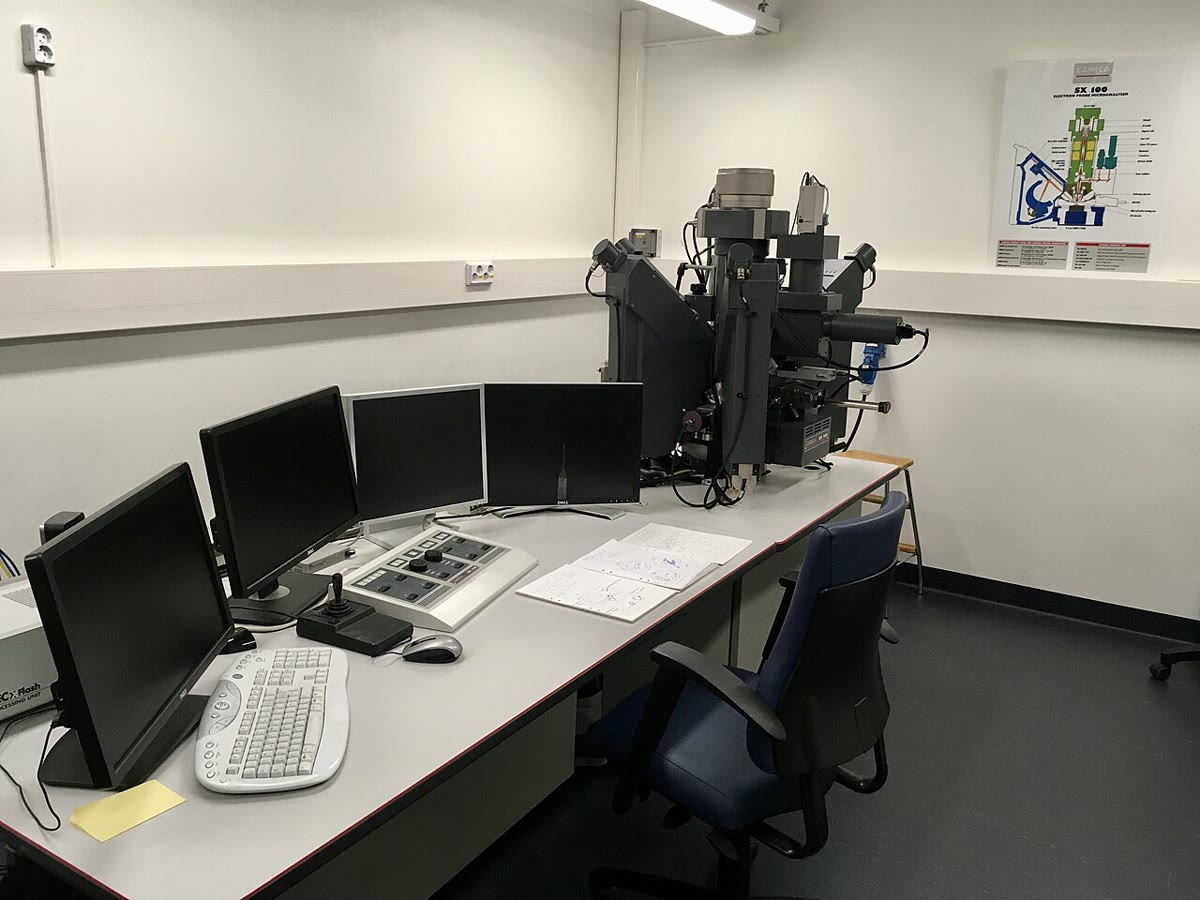
\includegraphics[width=\linewidth]{images/book4/b2-31-microprobe.jpg}
\par\smallskip{\scriptsize \omterm{def:b2:field-lab-methods-2:epma}{Mikroprobe elektron}: kolom elektron, dengan spektrometer-spektrometernya
di sekelilingnya, dan meja operator. Foto Kallerna, CC BY-SA 4.0 (Wikimedia Commons).}
\end{minipage}
\end{inthelab}
% ledger: sercE:epma-spot, sercE:coating, photo:b2-31-microprobe

\section{Analisis isotop}\label{sec:b2:field-lab-methods-2:isotopes}

\omterm{def:b2:isotope-geochemistry:tracer}{Pelacak isotop radiogenik} dan umur (\cref{ch:b2:isotope-geochemistry}) bertumpu pada rasio yang diukur
sampai 0.01--\qty{0.001}{\percent}, pada unsur-unsur yang dipisahkan dari batuan melalui pelarutan
dan kromatografi pertukaran ion di laboratorium bersih, dengan udara tersaring (biasanya Kelas 100 sampai
1000) sehingga debu tidak menambahkan apa pun pada jumlah kecil yang dianalisis.
% ledger: sercT:tims

\begin{definition}[Spektrometri massa ionisasi termal, ICP-MS multikolektor, bias massa]\label{def:b2:field-lab-methods-2:tims}
Dalam \emph{spektrometri massa ionisasi termal}\index{spektrometri massa ionisasi termal} (TIMS), suatu
unsur yang dimurnikan dimuat pada pita logam tipis dan diionkan dengan memanaskannya dalam vakum; ion-ionnya
dipercepat melintasi beda potensial sampai \qty{10}{kV}, dipisahkan menurut massa dalam sektor magnetik,
dan dikumpulkan. Dalam \emph{ICP-MS multikolektor}\index{ICP-MS multikolektor}, ion-ion berasal dari
plasma gandeng induktif, yang mengionkan unsur-unsur yang sukar diionkan secara termal, dan beberapa
kolektor mengukur berkas-berkas bermassa berbeda pada saat yang sama. Yang disebut \emph{bias
massa}\index{bias massa} suatu pengukuran adalah penyimpangan rasio isotop terukur dari rasio
sebenarnya sampel yang disebabkan oleh instrumen, yang meneruskan atau mengionkan satu massa lebih mudah daripada
massa lainnya.
\end{definition}
% ledger: sercT:tims, sercM:mcicpms

Kedua instrumen mencapai presisi ini. TIMS umumnya mengionkan kurang dari
\qty{1}{\percent} atom, dan \omterm{def:b2:field-lab-methods-2:tims}{bias massanya} berubah terus-menerus selama satu pengukuran. Bias itu dikoreksi dengan menetapkan rasio dua isotop yang tidak
diubah oleh peluruhan apa pun, yang memerlukan unsur dengan sedikitnya tiga isotop, dua di antaranya stabil dan bukan
radiogenik. Untuk stronsium, $^{86}\mathrm{Sr}/^{88}\mathrm{Sr}$ ditetapkan pada 0.1194, dan salah satu
bentuk koreksi yang umum adalah hukum eksponensial.
% ledger: sercT:tims, sercM:mcicpms, cheong14:mass-bias, ciaaw:sr-isotopes

\begin{proposition}[Hukum eksponensial bias massa]\label{prop:b2:field-lab-methods-2:bias}
Andaikan setiap rasio terukur dua isotop bermassa $m_i$ dan $m_j$ berhubungan dengan rasio
sebenarnya melalui $R_{ij}^{\mathrm{true}} = R_{ij}^{\mathrm{meas}}\,(m_i/m_j)^{\beta}$, dengan satu eksponen
$\beta$ untuk seluruh pengukuran. Maka rasio terukur $r$ suatu pasangan acuan, yang nilai sebenarnya
$r_0$ diketahui, memberikan
\begin{equation}
\beta = \frac{\ln(r_0/r)}{\ln(m_k/m_l)}
\label{eq:b2:field-lab-methods-2:beta}
\end{equation}
untuk pasangan acuan $k/l$, dan setiap rasio lain dikoreksi dengan $\beta$ yang sama.
\end{proposition}

\begin{proof}
Bila diterapkan pada pasangan acuan, hukum itu berbunyi $r_0 = r\,(m_k/m_l)^\beta$; dengan mengambil logaritma,
$\ln(r_0/r) = \beta\ln(m_k/m_l)$, yaitu \eqref{eq:b2:field-lab-methods-2:beta}. Menurut hipotesis, eksponen itu
sama untuk semua rasio dalam pengukuran tersebut, sehingga eksponen itu mengoreksi masing-masing rasio.
\end{proof}

Untuk stronsium, pasangan acuannya adalah $^{86}\mathrm{Sr}/^{88}\mathrm{Sr}$ dengan $r_0 = 0.1194$, dan
$^{87}\mathrm{Sr}/^{86}\mathrm{Sr}$ yang terkoreksi adalah rasio terukur dikalikan
$(m_{87}/m_{86})^\beta$. Kelimpahan CIAAW, \qty{9.86}{\percent} stronsium-86 dan
\qty{82.58}{\percent} stronsium-88, memberikan nilai yang sama. Setiap sesi juga menjalankan suatu \omterm{def:b2:isotope-geochemistry:standards}{standar acuan
isotop}: satu laboratorium mengukur $^{87}\mathrm{Sr}/^{86}\mathrm{Sr} = 0.710252 \pm
0.000007$ pada bahan acuan NBS~987 dalam tujuh pengukuran.
% ledger: cheong14:mass-bias, ciaaw:sr-isotopes

Rasio saja tidak memberikan konsentrasi. Untuk itu, sejumlah \emph{spike} yang diketahui, yaitu larutan
unsur itu yang diperkaya secara buatan pada satu isotop, dicampurkan dengan sampel yang telah dilarutkan sebelum
pengolahan kimia, dan rasionya diukur dalam campuran itu. Laboratorium-laboratorium TIMS memakainya baik untuk
konsentrasi maupun untuk rasio induk terhadap anak.
% ledger: sercT:tims

\begin{proposition}[Pengenceran isotop]\label{prop:b2:field-lab-methods-2:id}
Misalkan suatu sampel mengandung $N_x$ mol isotop acuan $b$ dan suatu spike mengandung $N_s$ mol isotop itu, dan misalkan
$R_x$, $R_s$, dan $R_m$ adalah rasio isotop kedua $a$ terhadap $b$ dalam sampel, spike, dan
campuran. Maka
\begin{equation}
N_x = N_s\,\frac{R_s - R_m}{R_m - R_x} .
\label{eq:b2:field-lab-methods-2:id}
\end{equation}
Galat relatif $\varepsilon$ pada $R_m$ memberi $N_x$ galat relatif $\mathcal{M}\varepsilon$,
dengan pembesaran galat
\begin{equation}
\mathcal{M} = \frac{R_m\,(R_s - R_x)}{(R_s - R_m)(R_m - R_x)} ,
\label{eq:b2:field-lab-methods-2:mag}
\end{equation}
yang terkecil ketika $R_m = \sqrt{R_s R_x}$.
\end{proposition}
\index{pengenceran isotop}

\begin{proof}
Isotop $a$ kekal dalam pencampuran: $R_m(N_x + N_s) = R_x N_x + R_s N_s$, sehingga $N_x(R_m - R_x) =
N_s(R_s - R_m)$, yaitu \eqref{eq:b2:field-lab-methods-2:id}. Turunan logaritmiknya adalah
$\mathrm{d}\ln N_x/\mathrm{d}\ln R_m = R_m\,[-1/(R_s - R_m) - 1/(R_m - R_x)] = -\mathcal{M}$, dengan
$\mathcal{M}$ seperti pada \eqref{eq:b2:field-lab-methods-2:mag}. Sampai konstanta positif $R_s - R_x$,
$1/\mathcal{M} = (R_s - R_m)(R_m - R_x)/R_m = R_s + R_x - R_m - R_sR_x/R_m$, yang turunannya
$-1 + R_sR_x/R_m^2$ lenyap pada $R_m = \sqrt{R_sR_x}$, suatu maksimum $1/\mathcal{M}$.
\end{proof}

\omterm{prop:b2:field-lab-methods-2:id}{Pengenceran isotop} tidak memerlukan garis kalibrasi maupun perolehan kembali unsur yang lengkap selama
pengolahan kimia: begitu spike dan sampel tercampur, kehilangan mengenai keduanya secara sama. Suatu spike stronsium
yang diterbitkan, misalnya, mengandung \qty{99.65}{\percent} stronsium-84, dengan
$^{84}\mathrm{Sr}/^{88}\mathrm{Sr} = 561.4$ dan $^{86}\mathrm{Sr}/^{88}\mathrm{Sr} = 0.7661$, pada
\qty{15.271}{\micro\gram} stronsium per gram larutan. Rasio 86/88-nya menunjukkan mengapa \omterm{def:b2:field-lab-methods-2:tims}{bias
massa} suatu campuran ber-spike tidak dapat dikoreksi dengan menetapkan $^{86}\mathrm{Sr}/^{88}\mathrm{Sr}$ pada
nilai alaminya: spike itu telah menggeser rasio tersebut.
% ledger: cheong14:spike, cheong14:mass-bias

\section{Kampanye pemetaan di inlier Varden}\label{sec:b2:field-lab-methods-2:campaign}

Di inti antiklin Varden, erosi telah memotong selubung batu pasir dan menyingkapkan
batuan dasar: sekis yang diterobos granit. Kampanye yang akan memasok laboratorium dimulai di
lapangan. Dua lintasan ditempuh dari barat ke timur melintasi inlier itu, dengan satu stasiun setiap
\qty{100}{m}; di setiap stasiun satuannya dicatat, dan sampel segar diambil di tempat batuan itu
tidak lapuk, diberi nomor sesuai stasiun, dan, bila fabrik akan diukur, diorientasikan. Gambar
memperlihatkan apa yang dijumpai stasiun-stasiun itu: dari 30 stasiun, sepuluh berada di granit, sepuluh di selubung batu pasir, satu di
sekis, satu di batu gamping, dan delapan di aluvium dasar lembah, tempat tidak ada batuan yang
tersingkap.

\begin{omfigure}
\centering
\begin{tikzpicture}
\begin{axis}[axis equal image, xmin=2.4, xmax=4.6, ymin=3.1, ymax=5.0, width=0.66\linewidth,
  tick label style={font=\scriptsize}, xlabel={timur (km)}, ylabel={utara (km)},
  label style={font=\small}]
% units: figdata/shared/region.py (read only); stations: figdata/bachelor-2/labmethods.py part stations
\addplot[lith schist, draw=black, line width=0.3pt, even odd rule] table {figdata/out/shared-region-unit-schist.dat};
\addplot[lith granite, draw=black, line width=0.3pt, even odd rule] table {figdata/out/shared-region-unit-granite.dat};
\addplot[om lith={icsTriassic!35}{om sand}, draw=black, line width=0.3pt, even odd rule] table {figdata/out/shared-region-unit-sandstone.dat};
\addplot[om lith={icsJurassic!40}{om limestone}, draw=black, line width=0.3pt, even odd rule] table {figdata/out/shared-region-unit-limestone.dat};
\addplot[om lith={icsJurassic!15}{om shale}, draw=black, line width=0.3pt, even odd rule] table {figdata/out/shared-region-unit-shale.dat};
\addplot[lith alluvium, draw=black, line width=0.3pt, even odd rule] table {figdata/out/shared-region-unit-alluvium.dat};
\addplot[river] table {figdata/out/shared-region-river.dat};
\addplot[only marks, mark=*, mark size=1.6pt, mark options={fill=white, draw=black}]
  table[x=x_km, y=y_km] {figdata/out/bachelor-2-labmethods-stations.dat};
\addplot[only marks, mark=*, mark size=1.6pt, mark options={fill=omThm, draw=black},
  x filter/.expression={\thisrow{unit}==2 ? x : nan}]
  table[x=x_km, y=y_km] {figdata/out/bachelor-2-labmethods-stations.dat};
\node[font=\scriptsize, fill=white, inner sep=1pt, anchor=east] at (axis cs:2.76,3.7) {1};
\node[font=\scriptsize, fill=white, inner sep=1pt, anchor=west] at (axis cs:4.24,3.7) {15};
\node[font=\scriptsize, fill=white, inner sep=1pt, anchor=east] at (axis cs:2.76,4.4) {16};
\node[font=\scriptsize, fill=white, inner sep=1pt, anchor=west] at (axis cs:4.24,4.4) {30};
\draw[black, line width=0.5pt] (axis cs:3.5,4.44) -- (axis cs:3.5,4.62);
\node[font=\scriptsize, fill=white, inner sep=1pt, anchor=south] at (axis cs:3.5,4.62) {stasiun 23};
\pic at (axis cs:4.45,4.75) {northarrow};
\end{axis}
\end{tikzpicture}
\par\smallskip{\small Inlier batuan dasar Perbukitan Varden dengan 30 stasiun dari dua lintasan barat--timur,
yang berjarak \qty{100}{m}. Titik merah: stasiun di granit. Merah muda dengan tanda silang: granit; abu-abu: sekis; ungu: batu pasir
Trias; biru: batu gamping Jura; biru pucat: serpih Jura; krem: aluvium sungai, yang
mengalir ke timur. Sampel
granit untuk soal akhir pekan berasal dari stasiun 23.}
\end{omfigure}

\begin{inthefield}[Pengambilan sampel untuk laboratorium]
\centering
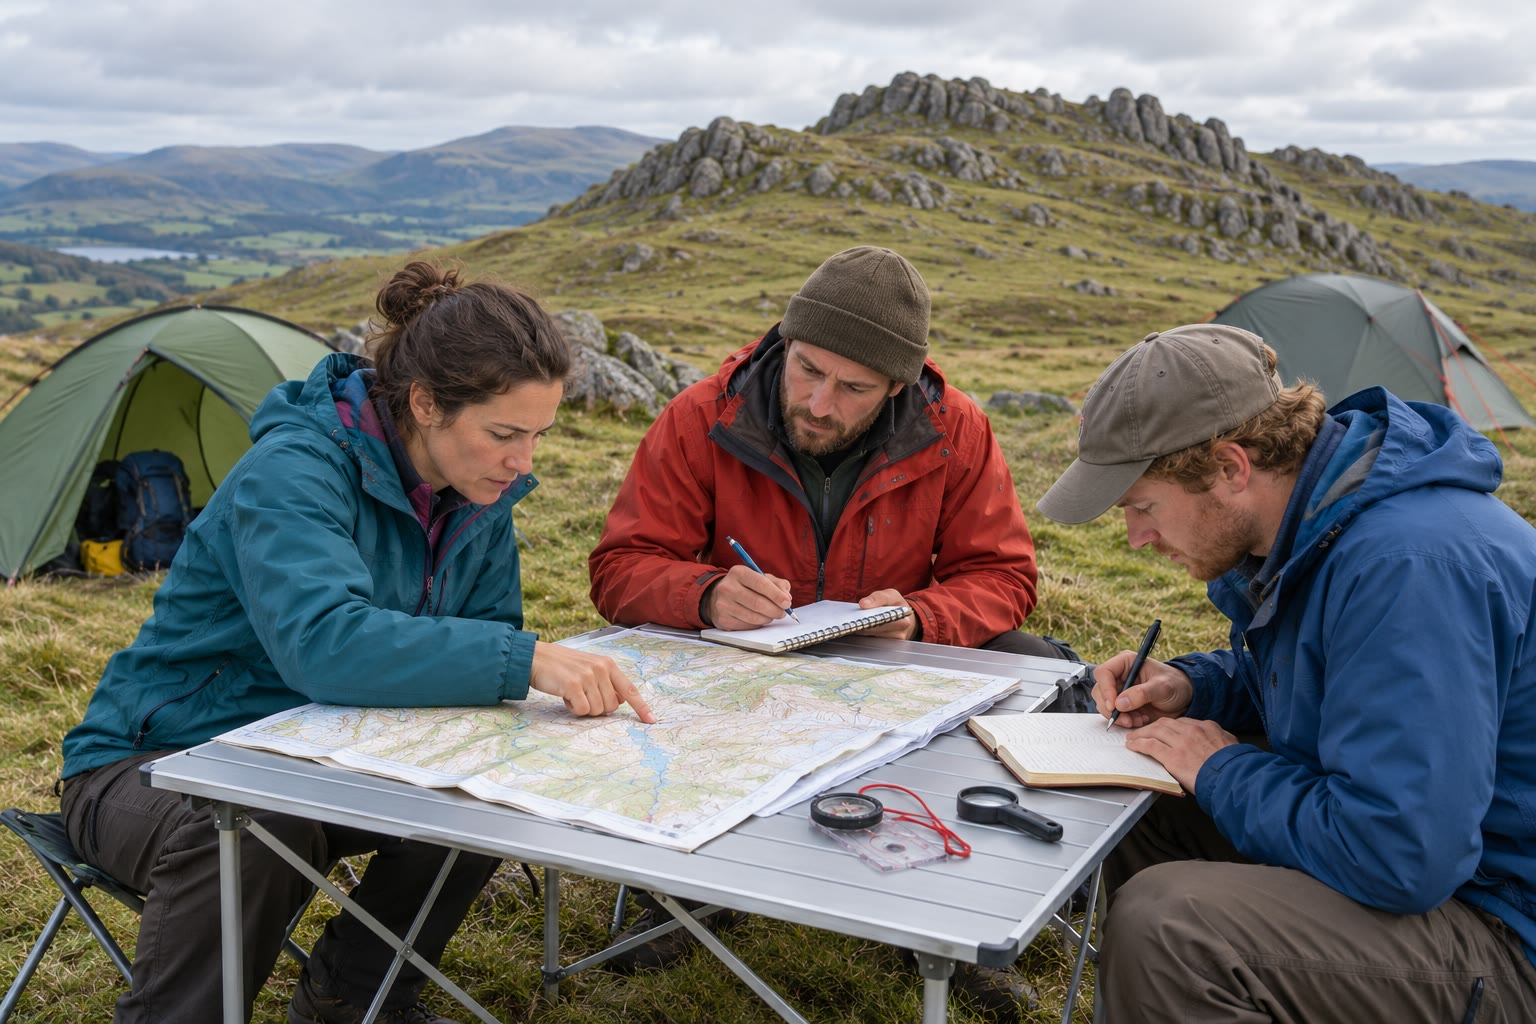
\includegraphics[width=0.56\linewidth]{images/book4/ai/b2-field-camp.jpg}
\par\smallskip{\small Satu regu lapangan merencanakan lintasan hari berikutnya (ilustrasi buatan AI).}
\par\medskip\raggedright
Pada malam hari regu itu memindahkan stasiun-stasiun ke peta, memeriksa bahwa setiap nomor sampel dalam
buku catatan cocok dengan sebuah kantong, dan memutuskan sampel mana yang dikirim ke laboratorium mana. Satu sampel dari setiap satuan
dikirim ke laboratorium sayatan tipis; granit dan sekis yang paling segar dikirim
untuk dihancurkan dan dianalisis sebagai batuan utuh; beberapa sampel granit disisihkan untuk isotop. Nomor
stasiun mengikuti setiap sampel melalui setiap langkah, dari kantong ke sayatan tipis,
serbuk, manik, dan baris suatu tabel data, sehingga setiap hasil yang ganjil dapat dilacak kembali ke
singkapannya.
\end{inthefield}

\section{Mutu suatu angka}\label{sec:b2:field-lab-methods-2:quality}

Setiap langkah dalam rangkaian itu menambahkan galatnya sendiri, dan metode-metode bab ini memperlihatkan dua jenis galat yang
dibedakan oleh buku-buku kimia. \omterm{def:b2:field-lab-methods-2:modal}{Penghitungan titik} dan rasio isotop kebanyakan memiliki galat acak, yang
mengecil ketika cacahan bertambah, seperti $1/\sqrt n$; kalibrasi memiliki galat sistematis, yang tidak berkurang dengan
pengulangan dan yang hanya terungkap oleh bahan acuan. Gambar analisis silika memperlihatkan
keduanya: batang-batangnya adalah presisi metode, dan titik yang meleset dari nol sebanyak berkali-kali batangnya
dibagi akar kuadrat banyaknya analisis adalah suatu bias. Unsur yang sama yang diukur dengan dua
metode, stronsium dengan XRF dan dengan \omterm{prop:b2:field-lab-methods-2:id}{pengenceran isotop}, merupakan pemeriksaan tambahan, karena keduanya tidak berbagi
kalibrasi. Hasil dilaporkan bersama ketidakpastiannya, dibulatkan menurut ketidakpastian itu, dan bersama bahan
acuan yang dijalankan bersamanya; angka tanpa keduanya tidak dapat dibandingkan dengan angka lain mana pun.

\section*{Latihan}\label{sec:b2:field-lab-methods-2:exercises}

Data untuk latihan, kecuali dinyatakan lain: massa atom H 1.008, O 15.999, Mg 24.305, Al
26.982, Si 28.085, K 39.098, Sr 87.62; massa isotop $^{86}\mathrm{Sr}$ 85.909261,
$^{87}\mathrm{Sr}$ 86.908878, $^{88}\mathrm{Sr}$ 87.905612; stronsium alam
$^{84}\mathrm{Sr}/^{86}\mathrm{Sr} = 0.05680$, \qty{9.86}{\percent} $^{86}\mathrm{Sr}$; spike
dalam teks, $^{84}\mathrm{Sr}/^{86}\mathrm{Sr} = 732.8$, \qty{0.13599}{\percent}
$^{86}\mathrm{Sr}$, berat atom 83.9242, \qty{15.271}{\micro\gram\per\gram}. Bulatkan sampai tiga
angka penting kecuali dinyatakan lain.
% ledger: ciaaw:H, ciaaw:O, ciaaw:Mg, ciaaw:Al, ciaaw:Si, ciaaw:K, ciaaw:sr-isotopes, cheong14:spike

\begin{exercise}[$\star$]\label{exo:b2:field-lab-methods-2:1}
(a) Sebutkan tekstur atau kristalnya: (i) dolerit yang bilah-bilah plagioklasnya seluruhnya terlingkupi dalam
kristal-kristal augit yang besar; (ii) marmer dengan butir-butir kalsit berukuran sama yang batas-batas lurusnya bertemu
bertiga; (iii) kristal staurolit sepanjang \qty{5}{mm} yang penuh inklusi kuarsa dalam sekis mika;
(iv) garnet yang dikelilingi tepian plagioklas dan piroksen yang menerus. (b) Tiga batas butir
bertemu pada \ang{104}, \ang{128}, dan \ang{128}. Tentukan rasio tegangan batas yang menghadap
sudut \ang{104} terhadap tegangan batas-batas lainnya.
\end{exercise}

\begin{exercise}[$\star$]\label{exo:b2:field-lab-methods-2:2}
Suatu batuan berbutir kasar mengandung \qty{25}{\percent} kuarsa, 15 feldspar alkali, 40 plagioklas, 12
biotit, dan 8 hornblende. (a) Hitung ulang Q, A, dan P. (b) Tentukan P/(A+P) dan namai batuan itu. (c) Tentukan
indeks warnanya dan golongkan batuan itu.
\end{exercise}

\begin{exercise}[$\star$]\label{exo:b2:field-lab-methods-2:3}
Penghitungan 800 titik mendapati suatu mineral sebesar \qty{12}{\percent}. (a) Tentukan simpangan baku
proporsi ini, dan nilai relatifnya. (b) Berapa nilainya dengan 3200 titik?
\end{exercise}

\begin{exercise}[$\star$]\label{exo:b2:field-lab-methods-2:4}
Serbuk seberat \qty{0.8000}{g} beratnya menjadi \qty{0.7712}{g} setelah pemijaran, dan residunya dileburkan dengan
\qty{8.0000}{g} fluks. (a) Tentukan \omterm{def:b2:field-lab-methods-2:xrf}{hilang pijarnya}. (b) Tentukan fraksi massa sampel di dalam
manik. (c) Kacanya mengandung \qty{5.20}{\percent} \ce{SiO2}. Tentukan silika serbuk yang telah dipijarkan
dan silika serbuk semula.
\end{exercise}

\begin{exercise}[$\star\star$]\label{exo:b2:field-lab-methods-2:5}
(a) Berapa titik yang diperlukan untuk mengukur mineral aksesori yang menyusun \qty{2}{\percent} suatu batuan
dengan galat baku relatif \qty{10}{\percent}? (b) Dan mineral yang menyusun \qty{30}{\percent},
dengan galat relatif yang sama? (c) Berikan komentar tentang usaha yang dituntut oleh mineral yang jarang.
\end{exercise}

\begin{exercise}[$\star\star$]\label{exo:b2:field-lab-methods-2:6}
Dalam hasil USGS pada gambar, riolit RGM-1 memberikan \ce{SiO2} $= 72.89$ dengan simpangan
baku 0.19 dalam 20 analisis (rekomendasi 73.45), dan basal BCR-2 memberikan 54.17 dengan 0.13 dalam
20 analisis (rekomendasi 54.1). (a) Tentukan perolehan kembali masing-masing, dalam persen. (b) Tentukan simpangan
baku setiap rata-rata, dan nyatakan setiap selisih dari nilai rekomendasi dalam satuan simpangan baku itu.
(c) Hasil manakah yang memperlihatkan bias? Apakah metode itu kurang presisi untuk RGM-1?
\end{exercise}

\begin{exercise}[$\star\star$]\label{exo:b2:field-lab-methods-2:7}
Suatu analisis mikroprobe flogopit murni, $\mathrm{KMg_3AlSi_3O_{10}(OH)_2}$, akan diperiksa.
(a) Tentukan massa molar rumus itu dan fraksi massa \ce{H2O} yang dikandungnya. (b) Tentukan
fraksi massa \ce{K2O}, \ce{MgO}, \ce{Al2O3}, dan \ce{SiO2}, serta total yang akan diberikan analisis
yang eksak. (c) Mengapa total sekitar \qty{96}{\percent} untuk suatu mika bukan analisis yang buruk?
\end{exercise}

\begin{exercise}[$\star\star$]\label{exo:b2:field-lab-methods-2:8}
Suatu pengukuran TIMS pada standar stronsium memberikan $^{86}\mathrm{Sr}/^{88}\mathrm{Sr} = 0.11905$ dan
$^{87}\mathrm{Sr}/^{86}\mathrm{Sr} = 0.71062$. (a) Tentukan eksponen $\beta$ hukum eksponensial.
(b) Koreksilah rasio $^{87}\mathrm{Sr}/^{86}\mathrm{Sr}$, sampai lima desimal. (c) Isotop ringan atau
isotop beratkah yang diunggulkan dalam pengukuran itu?
\end{exercise}

\begin{exercise}[$\star\star$]\label{exo:b2:field-lab-methods-2:9}
Untuk memeriksa \omterm{prop:b2:field-lab-methods-2:id}{pengenceran isotopnya}, suatu laboratorium memberi spike pada \qty{0.0500}{g} basal acuan BHVO-2
dengan \qty{0.1000}{g} spike dalam teks, dan mengukur $^{84}\mathrm{Sr}/^{86}\mathrm{Sr} =
0.874$ dalam campuran itu. (a) Tentukan jumlah mol $^{86}\mathrm{Sr}$ dalam alikuot spike. (b) Tentukan
jumlah mol $^{86}\mathrm{Sr}$ dalam sampel, dan konsentrasi stronsiumnya dalam ppm. (c) Bandingkan dengan
nilai rekomendasi \qty{394.1}{ppm}.
\end{exercise}

\begin{exercise}[$\star\star\star$]\label{exo:b2:field-lab-methods-2:10}
Untuk spike stronsium dalam teks ($R_s = 732.8$, $R_x = 0.05680$): (a) tentukan rasio campuran
yang meminimumkan pembesaran galat, dan nilai pembesaran itu di sana; (b) hitunglah $\mathcal M$ pada
$R_m = 0.1$, 0.5, 1.664, dan 100; (c) jelaskan mengapa campuran yang dekat dengan salah satu anggota ujung harus
dihindari, dan seberapa besar keleluasaan analis dalam praktik.
\end{exercise}

\begin{exercise}[$\star\star\star$]\label{exo:b2:field-lab-methods-2:11}
Penghitungan pada suatu granit mendapati 400 titik feldspar, \qty{62}{\percent} di antaranya plagioklas. (a) Dengan memperlakukan
plagioklas di antara titik-titik feldspar sebagai cacahan binomial, tentukan simpangan baku
P/(A+P). (b) Seberapa jauh hasil itu dari batas granodiorit, dalam simpangan baku? (c) Berapa
titik feldspar yang akan menempatkannya dua simpangan baku dari batas itu?
\end{exercise}

\begin{exercise}[$\star\star\star$]\label{exo:b2:field-lab-methods-2:12}
Suatu mineral menempati fraksi $p$ suatu batuan. (a) Tunjukkan bahwa probabilitas $n$ titik yang saling bebas
semuanya meleset darinya adalah $(1-p)^n$. (b) Berapa titik yang memberikan peluang sedikitnya \qty{95}{\percent} untuk
mengenai sedikitnya sekali mineral yang menyusun \qty{1}{\percent} batuan? (c) Hal yang sama untuk zirkon pada
\qty{0.05}{\percent}, dan simpulkan bagaimana suatu mineral aksesori sebaiknya dicari.
\end{exercise}

\section*{Soal akhir pekan}

\begin{problem}[{Soal akhir pekan --- Dari singkapan ke analisis}]\label{pb:b2:field-lab-methods-2:1}
% invented sample; data: ledger rows below; values: calc/ch31.py
Sampel VH-23 dari granit Varden diambil di stasiun 23 kampanye itu. Satu sayatan tipis
dihitung titiknya pada kisi teratur 1200 titik: kuarsa 372, feldspar alkali 348, plagioklas 324,
biotit 108, muskovit 36, oksida opak 12. Serbuk seberat \qty{0.8000}{g} beratnya \qty{0.7949}{g}
setelah dipijarkan pada \qty{925}{\celsius} dan dileburkan dengan \qty{8.0000}{g} fluks. Manik dari tiga
bahan acuan memberikan intensitas \ce{SiO2} berikut (ribuan cacahan per detik, kcps): BCR-2,
rekomendasi \qty{54.1}{\percent}, 21.66; AGV-2, 59.3, 23.70; RGM-1, 73.45, 29.37; manik granit
memberikan 28.63. Oksida-oksida lain granit itu berjumlah \qty{27.15}{\percent}. Untuk isotop,
\qty{0.1000}{g} serbuk dilarutkan dan dicampur dengan \qty{0.2500}{g} spike dalam teks;
sampel dianggap memiliki kelimpahan stronsium alam seperti dalam latihan. Gunakan data
latihan.

\noindent\textbf{Bagian I --- Mode.}
\begin{enumerate}
  \item Tentukan proporsi modal setiap mineral.
  \item Tentukan simpangan baku proporsi kuarsa, dan simpangan baku relatif
        proporsi muskovit.
  \item Tentukan $M$ dan indeks warna $M'$, dan golongkan batuan itu.
  \item Hitung ulang Q, A, dan P menjadi berjumlah 100.
  \item Tentukan P/(A+P) dan namai batuan itu pada \omterm{def:b2:magmatic-series:qapf}{diagram QAPF}.
  \item Dengan simpangan baku binomial P/(A+P) atas 672 titik feldspar, apakah nama itu
        meyakinkan?
  \item Berapa titik yang akan menurunkan simpangan baku proporsi kuarsa menjadi satu
        poin persentase?
\end{enumerate}

\noindent\textbf{Bagian II --- Silika dengan fluoresensi sinar-X.}
\begin{enumerate}[resume]
  \item Tentukan \omterm{def:b2:field-lab-methods-2:xrf}{hilang pijarnya}.
  \item Tentukan fraksi massa sampel di dalam manik, dan silika kaca jika
        serbuk yang telah dipijarkan mengandung \qty{72}{\percent}.
  \item Cocokkan garis kuadrat terkecil $c = aI + b$ melalui ketiga bahan acuan; berikan $a$ sampai
        empat desimal dan $b$ sampai dua desimal.
  \item Tentukan \ce{SiO2} granit itu, sampai dua desimal.
  \item Tentukan residu ketiga bahan acuan. Apakah garis itu memadai?
  \item Jumlahkan oksida-oksida dan \omterm{def:b2:field-lab-methods-2:xrf}{hilang pijar}. Apakah prosedur USGS akan mengulang analisis ini?
  \item Hitung ulang silika menjadi berjumlah 100 tanpa zat volatil.
\end{enumerate}

\noindent\textbf{Bagian III --- Bias massa.}
\begin{enumerate}[resume]
  \item Dari kelimpahan CIAAW, tentukan $^{86}\mathrm{Sr}/^{88}\mathrm{Sr}$ alam dan bandingkan
        dengan nilai yang dipakai untuk normalisasi.
  \item Suatu alikuot tanpa spike memberikan $^{86}\mathrm{Sr}/^{88}\mathrm{Sr} = 0.11853$. Tentukan $\beta$ sampai
        empat desimal.
  \item Alikuot itu memberikan $^{87}\mathrm{Sr}/^{86}\mathrm{Sr} = 0.71655$. Koreksilah, sampai lima desimal.
  \item Tentukan bias per satuan massa, dalam persen.
  \item Mengapa koreksi ini tidak dapat dilakukan pada campuran ber-spike di Bagian IV?
\end{enumerate}

\noindent\textbf{Bagian IV --- Pengenceran isotop.}
\begin{enumerate}[resume]
  \item Periksalah bahwa spike itu mengandung \qty{99.65}{\percent} stronsium-84 dan \qty{0.13599}{\percent}
        stronsium-86.
  \item Tentukan jumlah mol stronsium dan $^{86}\mathrm{Sr}$ dalam alikuot spike, sampai empat
        angka penting.
  \item Periksalah nilai $R_s = 732.8$ dan $R_x = 0.05680$ dalam latihan.
  \item Rasio terkoreksi campuran itu adalah $R_m = 1.6812$. Tentukan jumlah mol $^{86}\mathrm{Sr}$
        dalam sampel.
  \item Tentukan pembesaran galatnya. Dengan $R_m$ diketahui sampai \qty{0.01}{\percent} dan konsentrasi spike
        sampai $\pm\qty{0.031}{\micro\gram\per\gram}$, tentukan ketidakpastian relatif
        hasilnya.
  \item Tentukan konsentrasi stronsium granit Varden, dalam ppm.
\end{enumerate}
\end{problem}
% ledger: bgsI:qapf, bgsI:colour-index, usgsT:procedure, usgsT:sio2-table, ciaaw:sr-isotopes, cheong14:spike, cheong14:mass-bias
